\chapter{Brain Teasers}

\section{Carré magique $3\times 3$}

\subsection*{Exercice :}

\begin{exerciseBox}[Carré magique $3\times 3$]
Un \emph{carré magique} d'ordre $3$ est une grille $3\times 3$ contenant les entiers $1$ à $9$ chacun une seule fois, telle que la somme de chaque ligne, de chaque colonne et des deux diagonales soit la même.
\medskip

\textbf{Question :}  Combien existe-t-il de carrés magiques distincts d’ordre $3$ ?

\end{exerciseBox}

\subsection*{Solution :}



Dans un carré magique $3\times 3$ utilisant $\{1,\dots,9\}$, la somme totale vaut
\[
1+2+\cdots+9=45.
\]
Comme il y a $3$ lignes de même somme, la \emph{constante magique} est
\[
M=\frac{45}{3}=15.
\]

On considère un carré générique
\[
\begin{pmatrix}
a_1 & a_2 & a_3 \\
a_4 & a_5 & a_6 \\
a_7 & a_8 & a_9
\end{pmatrix},
\qquad
\text{où } \{a_1,\dots,a_9\}=\{1,\dots,9\}.
\]

\medskip
\noindent\textbf{Observation clé : la case centrale.} 
On a : 
\[
\left\{
\begin{array}{l}
a_1 + \textcolor{red}{a_5} + a_9 = 15 \\
a_3 + \textcolor{red}{a_5} + a_7 = 15 \\
a_2 + \textcolor{red}{a_5} + a_8 = 15 \\
a_4 + \textcolor{red}{a_5} + a_6 = 15
\end{array}
\right.
\]
  

donc on voit bien la case $a_5$ appartient à toutes les sommes de ${a_1 , ..... , a_9}$


donc la seule valeur possible pour la case centrale est
\[
a_5=5.
\]

\medskip
\noindent\textbf{Conséquence : paires opposées.}
Les deux diagonales, les colonnes et les lignes passant par le centre imposent
\[
a_1+a_9=15-a_5=10,\quad
a_3+a_7=10,\quad
a_2+a_8=10,\quad
a_4+a_6=10.
\]
Ainsi, les $4$ paires disjointes qui doivent apparaître en positions opposées (par rapport au centre) sont exactement
\[
\{1,9\},\ \{2,8\},\ \{3,7\},\ \{4,6\}.
\]

\medskip
\noindent\textbf{Répartition coins / milieux d’arêtes.}
On montre (et c’est classique) que les nombres pairs $\{2,4,6,8\}$ doivent occuper les \emph{coins} et les nombres impairs extrêmes $\{1,3,7,9\}$ les \emph{milieux d’arêtes}. 
En effet, si un coin était occupé par un impair extrême (disons $1$), alors sa case opposée devrait être $9$ (pour sommer $10$), forçant des configurations incompatibles avec les sommes \(15\) sur les lignes et colonnes correspondantes. 
Cette contrainte est cohérente avec les paires ci-dessus et mène au schéma:
\[
\begin{array}{c}
\text{coins : } \{2,4,6,8\},\qquad
\text{milieux d’arêtes : } \{1,3,7,9\},\qquad
\text{centre : } 5.
\end{array}
\]

\medskip
\noindent\textbf{Complétion (exemple).}
Plaçons, sans perte de généralité (par symétries du carré), $8$ en haut à gauche. 
Alors la case opposée (bas droite) est $2$. 
En complétant les lignes/colonnes/diagonales à somme $15$ avec les paires ci-dessus, on obtient le carré 
\[
\begin{pmatrix}
8 & 1 & 6 \\
3 & 5 & 7 \\
4 & 9 & 2
\end{pmatrix},
\]
qui est bien magique (chaque ligne/colonne/diagonale somme à $15$).

\medskip
\noindent\textbf{Nombre de carrés magiques $3\times 3$.}

On travaille avec les entiers $\{1,\dots,9\}$ et constante magique $M=15$. On sait (voir solution précédente) que:
\begin{itemize}
  \item le centre vaut nécessairement $5$ ;
  \item les cases opposées par rapport au centre somment à $10$ ;
  \item les \emph{coins} contiennent exactement $\{2,4,6,8\}$ et les \emph{milieux d’arêtes} contiennent exactement $\{1,3,7,9\}$.
\end{itemize}

\medskip
\noindent\textbf{Étape 1 — Choix du coin de $2$ (4 possibilités).}
Plaçons le nombre $2$ dans un coin quelconque. Il y a $4$ coins, donc $4$ choix possibles.

\medskip
\noindent\textbf{Étape 2 — Choix de la position de $1$ (2 possibilités).}
une fois $2$ fixé à un coin, il existe exactement \emph{deux} façons admissibles de placer le $1$.

donc :
\[
\boxed{\ \#\{\text{carrés magiques }3\times 3\} \;=\; 4 \times 2 \;=\; 8\ }.
\]

voici tous les carrés magiques de taille $3 \times 3$ construits à partir de $\{1 , \dots , 9\}$

\[
\begin{array}{cccc}
\begin{pmatrix}
8 & 1 & 6\\
3 & 5 & 7\\
4 & 9 & 2
\end{pmatrix} &
\begin{pmatrix}
6 & 7 & 2\\
1 & 5 & 9\\
8 & 3 & 4
\end{pmatrix} &
\begin{pmatrix}
2 & 9 & 4\\
7 & 5 & 3\\
6 & 1 & 8
\end{pmatrix} &
\begin{pmatrix}
4 & 3 & 8\\
9 & 5 & 1\\
2 & 7 & 6
\end{pmatrix}
\\[20pt]
\begin{pmatrix}
6 & 1 & 8\\
7 & 5 & 3\\
2 & 9 & 4
\end{pmatrix} &
\begin{pmatrix}
4 & 9 & 2\\
3 & 5 & 7\\
8 & 1 & 6
\end{pmatrix} &
\begin{pmatrix}
8 & 3 & 4\\
1 & 5 & 9\\
6 & 7 & 2
\end{pmatrix} &
\begin{pmatrix}
2 & 7 & 6\\
9 & 5 & 1\\
4 & 3 & 8
\end{pmatrix}
\end{array}
\]


\section{Le problème des 5 pirates}

\subsection*{Exercice :}

\begin{exerciseBox}[Le problème des 5 pirates]
Cinq pirates, numérotés de $P_1$ (le plus âgé) à $P_5$ (le plus jeune), doivent se partager un trésor de $100$ pièces d’or.  
La procédure est la suivante :
\begin{itemize}
  \item Le pirate le plus âgé encore en vie propose un partage.
  \item Tous votent (lui inclus). En cas d’égalité, la proposition est acceptée.
  \item Si la proposition est rejetée, le pirate qui a proposé est jeté par-dessus bord, et on recommence avec les survivants.
\end{itemize}

\noindent Les pirates sont parfaitement rationnels et obéissent à trois principes :
\begin{itemize}
  \item Ils veulent avant tout \textbf{maximiser leur nombre de pièces}.
  \item S’il y a égalité, ils préfèrent \textbf{survivre}.
  \item S’il y a encore égalité, ils préfèrent jeter les autres pirates à la mer.
\end{itemize}

\medskip
\noindent \textbf{Question :} Quelle répartition des $100$ pièces propose $P_1$, et combien de pièces obtient chaque pirate ?
\end{exerciseBox}

\subsection*{Solution :}

On raisonne par \emph{récurrence inversée} (backward induction).

\medskip
\textbf{Cas 1 : 1 pirate ($P_5$).}  
Il garde tout : $(0,0,0,0,100)$.

\medskip
\textbf{Cas 2 : 2 pirates ($P_4,P_5$).}  
$P_4$ propose $(100,0)$ : il vote pour, $P_5$ contre, égalité $\Rightarrow$ acceptée.

\medskip
\textbf{Cas 3 : 3 pirates ($P_3,P_4,P_5$).}  
Si $P_3$ est tué, reste $(100,0)$ pour $(P_4,P_5)$.  
$P_5$ sait qu’il recevra $0$.  
Donc $P_3$ peut acheter le vote de $P_5$ en lui donnant $1$: $(99,0,1)$.

\medskip
\textbf{Cas 4 : 4 pirates ($P_2,P_3,P_4,P_5$).}  
Si $P_2$ est tué, on est dans le cas précédent $(99,0,1)$.  
$P_4$ sait qu’il aura $0$.  
Donc $P_2$ s’assure du soutien de $P_4$ en lui donnant $1$: $(99,0,1,0)$.

\medskip
\textbf{Cas 5 : 5 pirates ($P_1,P_2,P_3,P_4,P_5$).}  
Si $P_1$ est tué, partage précédent $(99,0,1,0)$.  
$P_2$ obtient $99$, $P_4$ obtient $1$, les autres $0$.  

Donc $P_1$ doit acheter 2 votes supplémentaires pour avoir la majorité (3 sur 5).  
Il sait que $P_3$ et $P_5$ reçoivent $0$ si $P_1$ est tué.  
Il peut donc leur donner chacun $1$ pièce, et garder $98$.  

\[
(P_1,P_2,P_3,P_4,P_5) = (98,0,1,0,1).
\]

\medskip
\textbf{Réponse.}  
Le pirate le plus âgé $P_1$ propose :  
\[
\boxed{98 \text{ pièces pour lui, 1 pièce pour $P_3$, 1 pièce pour $P_5$, et 0 pour $P_2,P_4$}.}
\]



\section{Tigres et mouton}

\subsection*{Exercice :}

\begin{exerciseBox}[Tigres et mouton]
Sur une île magique, on place $n$ tigres et un mouton. Les tigres peuvent manger de l’herbe, mais préfèrent le mouton. Règles :
\begin{itemize}
  \item (A) À chaque fois, un seul tigre peut manger le mouton. S’il le mange, ce tigre se transforme immédiatement en mouton.
  \item (B) Tous les tigres sont parfaitement rationnels et veulent survivre.
\end{itemize}
Le mouton sera-t-il mangé ? Donner la réponse en fonction de $n$ et conclure pour $n=100$.
\end{exerciseBox}

\subsection*{Solution}
\textbf{Idée :} raisonnement par récurrence (rétrograde) sur $n$.

\paragraph{Cas de base.}

\begin{align*}
&n=1:\ \text{le tigre mange le mouton (il ne risque rien).}\\
&n=2:\ \text{aucun ne mange (qui mangerait deviendrait mouton et serait mangé).}    
\end{align*}
    
\paragraph{Hérédité.}
Supposons vrai jusqu’à $n-1$ : \emph{le mouton est mangé ssi le nombre de tigres est impair}.
\begin{itemize}
  \item Si $n$ est \textbf{impair}, un tigre peut manger : il devient mouton et il reste $n-1$ tigres, \textbf{pair}. Par l’hypothèse, avec un nombre pair de tigres, aucun ne mangera le nouveau mouton. \(\Rightarrow\) C’est sûr pour lui, donc \textbf{un tigre mange}.
  \item Si $n$ est \textbf{pair}, si un tigre mange il reste $n-1$ tigres, \textbf{impair} : par l’hypothèse, avec un nombre impair de tigres, l’un d’eux mangera le nouveau mouton (qui est l’ex-mangeur). \(\Rightarrow\) C’est dangereux, donc \textbf{personne ne mange}.
\end{itemize}

\paragraph{Conclusion.}
\[
\boxed{\ \text{Le mouton est mangé} \iff n \text{ est impair}\ }.
\]
Pour $n=100$ (pair), \textbf{le mouton n’est pas mangé}.

\section{River crossing}

\subsection*{Exercice :}

\begin{exerciseBox}[River crossing]
Quatre personnes $A,B,C,D$ doivent traverser une rivière sur un vieux pont qui ne supporte
qu'au plus deux personnes à la fois. Il fait nuit : on ne peut traverser sans la torche, et il n'y en a qu'une.
Lorsqu'ils traversent à deux, ils avancent à la vitesse du plus lent.
Les temps de traversée sont : $A=10$ min, $B=5$ min, $C=2$ min, $D=1$ min.
\emph{Quel est le temps minimal pour que tout le monde traverse ?}
\end{exerciseBox}

\subsection*{Solution :}

\begin{figure}[H]
    \centering
    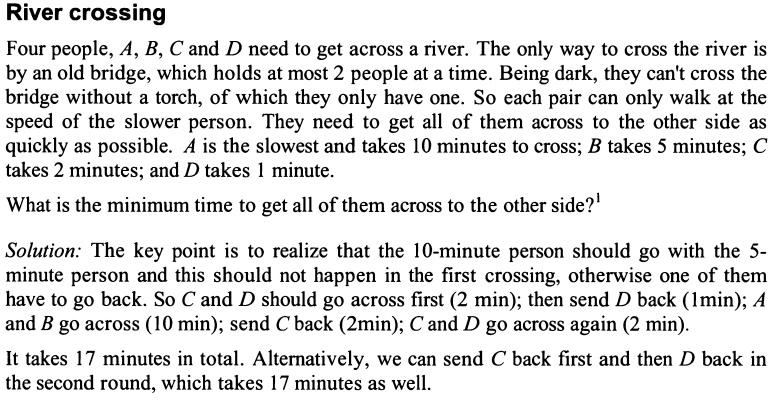
\includegraphics[width=0.75\linewidth]{exo_river.png}
    \caption{river crossing green book}
    \label{fig:placeholder}
\end{figure}



\section{Problème d’anniversaire}

\subsection*{Exercice :}

\begin{exerciseBox}[Problème d’anniversaire]
Toi et tes collègues savez que l’anniversaire de votre patron A est l’une des 10 dates suivantes :
\begin{itemize}
  \item \textbf{4 mars}, \textbf{5 mars}, \textbf{8 mars}
  \item \textbf{4 juin}, \textbf{7 juin}
  \item \textbf{1\up{er} septembre}, \textbf{5 septembre}
  \item \textbf{1\up{er} décembre}, \textbf{2 décembre}, \textbf{8 décembre}
\end{itemize}
A t’a dit \textbf{uniquement le mois} de son anniversaire, et il a dit à ton collègue C \textbf{uniquement le jour} (le chiffre).

Après cela, tu dis d’abord :
\begin{quote}
\og \textbf{Je ne connais pas} l’anniversaire de A ; \textbf{C ne le connaît pas non plus}. \fg
\end{quote}

Après t’avoir entendu, C répond :
\begin{quote}
\og \textbf{Je ne connaissais pas} l’anniversaire de A, \textbf{mais maintenant je le connais}. \fg
\end{quote}

Tu souris et dis alors :
\begin{quote}
\og \textbf{Moi aussi, maintenant je le connais}. \fg
\end{quote}

Après avoir regardé les 10 dates et entendu vos remarques, votre assistant administratif \textbf{a écrit la date d’anniversaire de A sans poser de question}.

\textbf{Question :} Quelle date l’assistant a-t-il écrite ?
\end{exerciseBox}

\subsection*{Solution}

\paragraph{Données filtrées par le premier énoncé.}
Tu sais que C ne peut pas connaître la date \emph{rien qu’avec le jour}. Les jours \emph{uniques} dans la liste sont
\[
\textbf{7} \ (\text{uniquement le } 7~\text{juin}) \quad \text{et} \quad \textbf{2} \ (\text{uniquement le } 2~\text{décembre}).
\]
Donc si le mois était \emph{juin} ou \emph{décembre}, il \emph{pourrait} arriver que C sache immédiatement (si le jour était 7 ou 2).
Comme tu affirmes que C ne peut pas savoir, le mois n’est \textbf{ni juin ni décembre}.
Il reste \textbf{mars} et \textbf{septembre} :
\[
\{\ 4~\text{mars},~5~\text{mars},~8~\text{mars},~1\up{er}~\text{sept.},~5~\text{sept.}\ \}.
\]

\paragraph{Après ton annonce, C sait maintenant.}
Dans l’ensemble restant, les jours qui identifient \emph{une date unique} sont
\[
1 \ (\text{seulement } 1\up{er}~\text{sept.}),\quad
4 \ (\text{seulement } 4~\text{mars}),\quad
8 \ (\text{seulement } 8~\text{mars}).
\]
Le jour \(\mathbf{5}\) reste ambigu (\(5~\text{mars}\) ou \(5~\text{sept.}\)).
Donc si C \emph{vient} de savoir, son jour n’est pas \(5\) : le jour est \(\mathbf{1}\), \(\mathbf{4}\) ou \(\mathbf{8}\).

\paragraph{Tu sais maintenant toi aussi.}
Si ton mois était \textbf{mars}, il resterait deux possibilités (4 mars ou 8 mars) et tu ne pourrais pas trancher.
Comme tu sais désormais, ton mois ne peut pas être mars : il est \textbf{septembre}.
Avec septembre et un jour dans \(\{1,4,8\}\), la seule date possible est \(\mathbf{1\up{er}~septembre}\).

\paragraph{Réponse.}
\[
\boxed{\text{1\up{er} septembre}}
\]





\section{Jeu de cartes}

\subsection*{Exercice :}

\begin{exerciseBox}[jeu de cartes]
Un casino propose un jeu de cartes utilisant un paquet normal de 52 cartes.
La règle est la suivante : on retourne deux cartes à la fois.
\begin{itemize}
    \item Si les deux cartes sont \textbf{noires}, elles vont dans la pile du croupier.
    \item Si les deux cartes sont \textbf{rouges}, elles vont dans votre pile.
    \item Si l’une est noire et l’autre rouge, elles sont écartées.
\end{itemize}
On répète l’opération jusqu’à épuisement des 52 cartes.  
Si vous avez plus de cartes dans votre pile que le croupier, vous gagnez \(\$100\); sinon (égalité comprise) vous ne gagnez rien.  
Le casino vous permet de négocier le prix d’entrée pour participer.  
Combien seriez-vous prêt à payer pour jouer à ce jeu ?
    
\end{exerciseBox}

\subsection*{Solution :}

Notons :

\[
\begin{cases}
n_{RR}=\text{nombre de paires (rouge, rouge)},\\
n_{BB}=\text{nombre de paires (noir, noir)},\\
n_{RB}=\text{nombre de paires (une rouge, une noire)}.    
\end{cases}
\]

Les paires \(RR\) vont dans \emph{votre} pile (2 cartes chacune), les paires \(BB\) dans la pile du croupier (2 cartes chacune), et les paires \(RB\) sont écartées.

En comptant les couleurs dans tout le paquet (52 cartes, donc 26 rouges et 26 noires), on obtient les identités
\[
2n_{RR}+n_{RB}=26 \qquad\text{(cartes rouges)}
\]
\[
2n_{BB}+n_{RB}=26 \qquad\text{(cartes noires)}.
\]
En soustrayant ces deux égalités, on trouve \(2n_{RR}=2n_{BB}\), donc
\[
n_{RR}=n_{BB}.
\]
Par conséquent, la taille de votre pile vaut \(2n_{RR}\) et celle du croupier vaut \(2n_{BB}\) : elles sont toujours égales, quel que soit l’ordre des cartes.

Ainsi, vous n’aurez \emph{jamais} strictement plus de cartes que le croupier; le résultat est toujours une égalité (ou, selon la règle, aucun gain pour vous). La valeur espérée du jeu est donc nulle, et le juste prix à payer pour jouer est
\[
\boxed{0}.
\]


\section{Deux cordes}

\subsection*{Exercice :}

\begin{exerciseBox}[deux cordes]
Vous disposez de deux cordes. Chacune prend exactement \textbf{1 heure} pour se consumer entièrement si on l’allume par une seule extrémité.  
Cependant, la vitesse de combustion n’est pas uniforme le long d’une corde (certaines sections brûlent plus vite que d’autres), de sorte qu’on ne peut pas supposer que la moitié de la corde prend 30 minutes à brûler, etc.  

En utilisant uniquement ces deux cordes et des allumettes, comment mesurer \textbf{45 minutes} ?
    
\end{exerciseBox}


\subsection*{Solution :}

Allumez simultanément \textbf{les deux extrémités de la première corde} et \textbf{une seule extrémité de la seconde corde}.  

\medskip
\noindent\textbf{Pourquoi ?}  
Allumer une corde par ses deux extrémités la fait brûler deux fois plus vite \emph{quelle que soit} l’irrégularité de densité : la durée totale est divisée par deux. Ainsi, la première corde se consume en \(\,30\,\) minutes.

\medskip
\noindent Après \(\,30\,\) minutes, la première corde est entièrement brûlée. À cet instant,
allumez \textbf{l’autre extrémité de la seconde corde}.  

Jusqu’ici, la seconde corde a brûlé pendant \(\,30\,\) minutes à partir d’une seule extrémité; il lui reste donc l’équivalent de \(\,30\,\) minutes de combustible (quelle que soit la répartition le long de la corde). En l’allumant maintenant par l’autre extrémité, la portion restante se consume deux fois plus vite : elle met \(\,30/2=15\,\) minutes à disparaître.

\medskip
\noindent Ainsi, le temps total écoulé est
\[
30 \text{ minutes} + 15 \text{ minutes} = \boxed{45 \text{ minutes}.}
\]


\section{Jeu en 2D}

\subsection*{Exercice :}

\begin{exerciseBox}[Jeu en 2D]
Dans un jeu en 2D, votre personnage est enfermé dans une grille \(6\times 6\).
Il démarre en \((0,0)\) (coin en bas à gauche) et ne peut se déplacer que vers le \textbf{haut}
ou vers la \textbf{droite}.  
Combien de chemins possibles mènent au point \((6,6)\) ?    
\end{exerciseBox}


\subsection*{Solution :}

Pour atteindre \((6,6)\) depuis \((0,0)\), il faut effectuer exactement
\(6\) déplacements vers la droite (\(R\)) et \(6\) vers le haut (\(U\)),
soit \(12\) pas au total.  
Chaque chemin correspond à une permutation de la suite de \(12\) mouvements
contenant \(6\) \(R\) et \(6\) \(U\).  
Le nombre de chemins est donc le coefficient binomial
\[
\binom{12}{6}=\frac{12!}{6!\,6!}=924.
\]
\[
\boxed{924}
\]

\begin{center}
% --------- Figure illustrative (TikZ) ---------
\begin{tikzpicture}[scale=0.6, line cap=round, line join=round]
  % Grille 6x6 (de (0,0) à (6,6))
  \draw[step=1cm,gray!50,thin] (0,0) grid (6,6);
  % Axes et étiquettes
  \draw[->,thick] (-0.3,0) -- (6.4,0) node[below right]{\small x};
  \draw[->,thick] (0,-0.3) -- (0,6.4) node[above left]{\small y};
  \node[below left] at (0,0) {\small (0,0)};
  \node[above right] at (6,6) {\small (6,6)};

  % Exemple de chemin (en gras bleu)
  \draw[very thick,blue,-{Latex[length=3mm]}]
    (0,0) -- (0,2) -- (3,2) -- (3,4) -- (6,4) -- (6,6);

  % Petites flèches pour indiquer les mouvements permis
  \draw[->,gray!80] (6.1,1) -- ++(0,0.8) node[right,black]{\small haut};
  \draw[->,gray!80] (5,-0.1) -- ++(0.8,0) node[below,black]{\small droite};
\end{tikzpicture}

\smallskip
\emph{Une grille \(6\times6\). En bleu, un chemin possible parmi \(924\).}
\end{center}



\section{Say 50}

\subsection*{Exercice :}

\begin{exerciseBox}[Say 50]
Vous et votre ami jouez à un jeu : chacun, à tour de rôle, choisit un entier
entre \(1\) et \(10\) (inclus) et l'ajoute à un total cumulatif.
Celui qui \emph{énonce} pour la première fois le nombre \(50\) gagne la partie.
Vous commencez. Quel nombre devez-vous dire en premier ?    
\end{exerciseBox}


\subsection*{Solution :}

L'idée est de se réserver des \emph{jalons} que l'on pourra toujours atteindre
quel que soit le coup adverse. Ici, comme chaque paire de coups
\((\text{adversaire} + \text{vous})\) peut totaliser au plus \(10+10\) mais,
surtout, vous pouvez toujours \emph{compléter à \(11\)} le nombre de l'adversaire,
les bons jalons sont les nombres espacés de \(11\).

Comme \(50 \equiv 6 \pmod{11}\), on vise la suite de jalons
\[
6,\;17,\;28,\;39,\;50 .
\]
\textbf{Stratégie gagnante.}
\begin{enumerate}
  \item Dites d'abord \(\boxed{6}\).
  \item Puis, après chaque nombre \(y\in\{1,\dots,10\}\) annoncé par l'adversaire,
        répondez \(\;11-y\). Le total augmente alors de \(y+(11-y)=11\)
        et passe successivement à \(17, 28, 39\) puis \(50\) \emph{à votre tour}.
\end{enumerate}

\paragraph{Justification formelle.}
Par récurrence, supposons que juste après votre tour le total vaut \(6+11k\)
pour un certain \(k\ge 0\). L'adversaire ajoute un \(y\in\{1,\dots,10\}\),
le total devient \(6+11k+y\). En répondant \(11-y\) (autorisé car
\(1\le 11-y\le 10\)), on obtient
\[
6+11k+y+(11-y)=6+11(k+1),
\]
c'est-à-dire le jalon suivant. Pour \(k=0,1,2,3\), on atteint finalement
\(6+11\cdot 4=50\) à votre cinquième coup. L'adversaire ne peut pas l'empêcher.

\medskip
\noindent\textbf{Réponse :} il faut dire \(\boxed{6}\) en premier.


\section{100 Ampoules}

\subsection*{Exercice :}

\begin{exerciseBox}[100 Ampoules]
Dans une pièce, il y a $100$ ampoules, chacune éteinte au départ, et disposant d’un interrupteur à son côté.

Le premier individu entre dans la pièce et actionne \textit{tous} les interrupteurs, allumant ainsi toutes les ampoules.
Le deuxième individu entre ensuite et actionne \textit{un interrupteur sur deux} (c’est-à-dire ceux des ampoules numérotées $2, 4, 6, \ldots, 100$).  
Le troisième individu entre et actionne \textit{un interrupteur sur trois} (ceux des ampoules $3, 6, 9, \ldots$).  

Le processus continue ainsi : le $n$-ième individu actionne chaque $n$-ième interrupteur, jusqu’à ce que le $100$-ième individu actionne uniquement le $100$-ième interrupteur.

\medskip
\textbf{Question :} Après le passage du $100$-ième individu, combien d’ampoules restent allumées ?
\end{exerciseBox}

\subsection*{Solution :}


\textbf{Idée générale.} On numérote les lampes de $1$ à $100$. La personne $k$ bascule \emph{toutes} les lampes dont le numéro est multiple de $k$.

\begin{enumerate}
  \item \textbf{Qui touche quelle lampe ?} 
  La personne $k$ agit sur la lampe $i$ si et seulement si  $k\mid i$. 
  Ainsi, la lampe $i$ est basculée autant de fois qu’elle a de diviseurs : soit $\tau(i)$.

  \item \textbf{Quand une lampe finit-elle allumée ?}
  Chaque bascule inverse l’état. Au final, la lampe $i$ est \emph{allumée} si et seulement si elle a été basculée un nombre \emph{impair} de fois, c’est-à-dire si $\tau(i)$ est impair.

  \item \textbf{Parité de $\tau(i)$ et carrés parfaits.}
  Les diviseurs de $i$ se couplent naturellement par paires $(d,\; i/d)$. 
  On obtient donc en général un nombre \emph{pair} de diviseurs. 
  L’unique cas où un couple se « confond » est lorsque $d=i/d$, soit $d^2=i$ : autrement dit, lorsque $i$ est un \emph{carré parfait}. 
  Ainsi, $\tau(i)$ est impair \emph{si et seulement si} $i$ est un carré parfait.

  \item \textbf{Application à $100$ lampes.}
  Les lampes allumées à la fin sont exactement celles d’indices carrés parfaits $\le 100$, 
  à savoir $1,4,9,16,25,36,49,64,81,100$. 
  Il y en a $\lfloor \sqrt{100}\rfloor = 10$.
\end{enumerate}

\[
\boxed{\,\text{Au final, } 10 \text{ lampes restent allumées.}\,}
\]

